\documentclass[landscape, a4paper]{article}
\usepackage[margin=0cm,top=0.4cm,bottom=0.4cm,left=0.4cm,right=0.4cm]{geometry}
% \usepackage[showframe,margin=0cm,top=0.5cm,bottom=0.5cm,left=0.5cm,right=0.5cm]{geometry}
\usepackage[export]{adjustbox}
\usepackage{xcolor}
\usepackage{caption}
\usepackage{csquotes}
\usepackage{titlesec}
\usepackage{etoolbox} % Add this to your preamble
\usepackage[parfill]{parskip}

\newtoggle{isEnglish}
\toggletrue{isEnglish}
% \togglefalse{isEnglish}

\captionsetup{labelformat=empty, justification=centering, font={color=PrimaryColor}}

\definecolor{PrimaryColor}{HTML}{f82f1c}
\newcommand\alert[1]{\textcolor{PrimaryColor}{\textbf{#1}}}

\titleformat{\section}
{\color{PrimaryColor}\normalfont\normalsize\bfseries}
{\thesection}{0.5cm}{}
\titlespacing{\section}{0cm}{0.2cm}{0.2cm}
% \renewcommand{\thesection}{\arabic{section}}

\titleformat{\subsection}
{\color{PrimaryColor}\normalfont\normalsize\bfseries}
{\thesubsection}{0.5cm}{}
\titlespacing{\subsection}{0cm}{0.1cm}{0.1cm}

\begin{document}
\noindent
\centering
\footnotesize
\begin{minipage}[t]{0.31\textwidth}
	\setlength{\parskip}{0.25cm}
	\vspace{0.5cm}

	\textcolor{PrimaryColor}{
		\rule{\linewidth}{0.5mm}
		\vspace{-0.1cm}
		\begin{center}
			\large
			\textsc{\iftoggle{isEnglish}{Hike through Hell's Valley}{}}
		\end{center}
		\rule{\linewidth}{0.5mm}
	}

	\iftoggle{isEnglish}{
    % The name "Höllental" dates back to the Middle Ages. Early records refer to it as "die Helle," a term which originally meant a bright or steep place, rather than connoting hell in the modern sense. Over time, linguistic shifts and the imposing, sometimes treacherous nature of the gorge transformed the name into "Höllental," interpreted as "Hell's Valley." The dark, narrow passages and high cliffs likely contributed to this dramatic rebranding, especially among travelers who experienced its dangers firsthand during bad weather.
    An exact person who named Hell's Valley is unknown, but the name developed over time in the Middle Ages, probably in the 13th or 14th century. The name \alert{\enquote{Höllental}} likely comes from old German words such as \enquote{Hölle}, meaning hell, because the valley is surrounded by steep cliffs and dense forest, and the valley felt dark, frightening, and wild, like a hellish place. Travelers got robbed there, and the paths were narrow and difficult to pass through, especially in winter and before modern roads existed. It may also stem from "helle" or "hal," ancient words for steep, narrow valley or rocky gorge. Luckily, the valley is now a beautiful tourist area with good roads and the famous Höllentalbahn railway.
	}{
	}

	\includegraphics[width=\linewidth]{./figures/höllental_resized.png}
	\captionof{figure}{\iftoggle{isEnglish}{View from the ruins of Falkenstein Castle into the Höllental}{}}
	\setlength{\parskip}{0.25cm}

	\iftoggle{isEnglish}{
    One of the most significant historical developments in the valley was the construction of the \alert{Höllentalbahn}, or Hell Valley Railway. The line was inaugurated in 1887, with the segment through Höllental initially operated using cogwheel technology due to the steep gradients. In 1936, the Deutsche Reichsbahn electrified the line between Freiburg and Neustadt.

    The railway line through the Höllental is not only one of the most scenic train routes in Germany, but also one of the steepest. Due to this extreme incline and the challenging topography, a \alert{special safety measure} must be implemented to ensure the secure operation of the trains. A second crew member must always be present in the train cab when ascending the Höllental. This measure is in place to ensure immediate human response in the event that the train driver becomes incapacitated, for example due to fainting or a sudden health issue. Although modern trains are equipped with automatic braking systems that would bring the train to a stop if the driver is unresponsive for a certain time, the speed at which a train could gain momentum on such a steep grade would make a delayed stop potentially dangerous. %The second crew member can intervene instantly if necessary, ensuring that the train is brought to a safe halt as quickly as possible.

	}{
	}
\end{minipage}%
\hfill%
\vrule width 0.01cm
\hfill%
\begin{minipage}[t]{0.31\textwidth}
	\vspace{0cm}
	\setlength{\parskip}{0.25cm}

	\iftoggle{isEnglish}{

    The \alert{\enquote{Hirschsprung}} is one of the most iconic and narrowest points in the Höllental, and it holds both geographical and legendary significance. The name \enquote{Hirschsprung} translates to stag leap. According to the story, a stag, pursued by hunters, managed to escape by leaping across the narrow gorge at this point, which measures about 9 meters wide at its narrowest part. A major transformation came with the construction of the Höllentalbahn railway. When the railway opened in 1887, engineers had to blast through rock and construct a narrow path along the valley wall near the Hirschsprung.
	}{
	}

	\includegraphics[width=\linewidth]{./figures/hirschsprung.png}
	\captionof{figure}{\iftoggle{isEnglish}{The stag monument today}{}}
	\setlength{\parskip}{0.25cm}

	\iftoggle{isEnglish}{
    Hell's Valley (Höllental) was most likely formed through a combination of geological processes that unfolded over millions of years. The valley's dramatic, steep-sided gorge is the result of both tectonic activity and glacial erosion, which together shaped the landscape into what we see today.

    The \alert{wind} that moves through the Höllental is shaped by the valley’s narrow, steep-sided topography, which acts like a natural wind tunnel. Air masses from the Upper Rhine Plain are funneled through the constricted valley corridor between steep rock faces and dense forest. As a result, the wind accelerates noticeably, especially when weather systems cause pressure differences between the Rhine Valley and the higher elevations of the Black Forest plateau near Hinterzarten.

A particularly striking phenomenon occurs in the evening hours. As the sun sets and the slopes of the valley begin to cool down, the air in the higher altitudes of the Black Forest also loses warmth. Cooler air is denser and tends to sink, while the warm air of the Rhine Plain remains lighter and more stable. This creates a suction effect toward the east, as the cooling air masses draw in warmer air from the lowlands. This pressure difference results in a steady, noticeable evening wind that flows up the valley, refreshing the air and offering natural ventilation even after hot summer days.

This channeled airflow does not only affect the microclimate within the valley itself. It also has a direct influence on the climate of the city of Freiburg, particularly in the districts that lie along the mouth of the Höllental such as Littenweiler, Waldsee and Oberau. The natural ventilation provided by the Höllental wind makes Freiburg’s climate slightly milder in extreme heat phases than in comparable cities without this kind of geographic advantage.
	}{
	}
\end{minipage}%
\hfill\color{white}%
\vrule width 0.01cm
\hfill\color{black}%
\begin{minipage}[t]{0.31\textwidth}
	\vspace{0cm}
	\setlength{\parskip}{0.25cm}

	\iftoggle{isEnglish}{
    The \alert{\enquote{Ravennaschlucht} (Ravenna Gorge)}, a side valley branching off from the Höllental near Hinterzarten in the Black Forest, is one of the region’s most striking natural and historical landmarks. Its name likely derives from the Old High German word \enquote{Rafan}, meaning raven, possibly referring to the birds that once populated the steep, forested cliffs or to the gorge’s dark and shadowy character.

    Visitors can explore the gorge itself by foot. The gorge trail, which includes small wooden bridges, rocky steps, and narrow paths, follows the course of the Ravenna brook and leads through dense forest past waterfalls and moss-covered rock faces. The most well-known waterfall, the \alert{Great Ravenna Fall}, plunges about 16 meters and is especially striking after rainfall or snowmelt.
	}{
	}

	\includegraphics[width=\linewidth]{./figures/ravenna_waterfall_resized.png}
	\captionof{figure}{\iftoggle{isEnglish}{Great Ravenna Fall}{}}
	\setlength{\parskip}{0.25cm}

	\iftoggle{isEnglish}{
    The \alert{\enquote{Kreuzfelsenkurve} (Cross Rock Curve)} is one of the most striking bends along the modern B31 road through the Höllental. It is named after the Kreuzfelsen, a prominent rock formation that towers above the curve and is easily recognizable due to the white cross mounted on its peak. %The name "Kreuzfelsen" dates back several centuries and likely has religious origins, as crosses were often erected in such places for spiritual protection and as markers for travelers navigating the steep and often dangerous valley paths.
	}{
	}

	\includegraphics[width=\linewidth]{./figures/kreuzfelsenkurve.png}
	\captionof{figure}{\iftoggle{isEnglish}{\enquote{Kreuzfelsenkurve} (cross rock curve)}{}}
	\setlength{\parskip}{0.25cm}

	\iftoggle{isEnglish}{
Before the construction of the modern B31 in the 20th century, the main route through the Höllental was a steep, narrow mule track known as the \alert{\enquote{Alte Steige} (Old Climb)}. This historic path led directly up the valley slope and was used for centuries by traders, travelers, and postal coaches to reach the Black Forest plateau. 
    % Historically, the Ravenna Gorge served as an important route for trade and travel through the mountains, despite its rugged terrain. Glassworks that were active from 1740, relied on the vast wood resources in the surrounding forests to fuel the furnaces, and the Ravenna brook provided the necessary water power. Remains of this glassmaking tradition can still be seen today in the area.
  }{}

\end{minipage}%
\newpage
\begin{minipage}[t]{0.31\textwidth}
	\vspace{0cm}
	\setlength{\parskip}{0.25cm}

	\iftoggle{isEnglish}{
Due to its steep incline and sharp turns, it required specially bred horses with great strength and sure-footedness. These horses were known as \alert{\enquote{Schwarzwälder Füchse} (Black Forest Foxes)}, a breed developed specifically in this region. With their sturdy build, calm temperament they were ideal for pulling loads up the difficult terrain. The \enquote{Alte Steige} remained the main connection between the Rhine Valley and the highlands until the growing demands of motorized traffic led to the planning of a modern road.
% , and reddish-brown coats, 

 %The B31 was gradually expanded and rerouted during the 20th century to follow a gentler, more navigable path through the valley, but sections like the Kreuzfelsenkurve still reflect the dramatic topography of the original route. The current curve near the Kreuzfelsen was engineered with significant effort to accommodate modern vehicles while preserving the natural rock formations and steep forest slopes.

% Today, the Kreuzfelsenkurve is not only a functional part of the B31 but also a visual highlight for travelers, offering views of the cliffs and forest and evoking the deep historical roots of transportation in the Höllental. The nearby remnants of the Alte Steige can still be hiked, allowing visitors to retrace the steps of travelers and draft horses who once made the steep ascent into the Black Forest using paths shaped by centuries of regional life and trade.

The \alert{\enquote{Posthalde}} is a historically significant stopover point along the old route through the valley. The name \enquote{Posthalde} refers to a place where mail coaches, or "Postkutschen," would pause, serving as a resting and switching point for horses, especially before tackling the demanding incline up the \enquote{Alte Steige}. When the Höllentalbahn was built, the Posthalde site was transformed into both a station and a transshipment point for goods and mail. %The station building, which still stands, was erected in 1887 to serve railway traffic through the valley. %The name “Posthalde” reflects its dual past as both a mail station and a steep roadside terrain feature. For centuries travelers and postal couriers from across Europe paused here. During Habsburg rule over Breisgau, starting in 1368, this section of the valley formed part of the Vienna–Paris postal route, and the Posthalde site served as a crucial relay and rest stop for Austrian couriers .
. %Situated between Himmelreich and Hinterzarten, it was first mentioned in the 15th century under the name “Wyhlers Gut.” By the mid-16th century, a post house had been established here. Over the centuries, it evolved into one of the three principal estates lining the Höllental, alongside Hofgut Sternen and Himmelreich .

 % The station remained in use until the 1970s, when passenger stops at Posthalde, Hirschsprung, and Höllsteig were all discontinued and the station buildings were sold into private hands .


 %Its layered roles—as postal stop, agricultural hub, railway station, and waypoint on scenic hiking routes—made the Posthalde a microcosm of Hell’s Valley’s broader history: a place shaped by nature, travel, and the continuous meeting of local tradition and international movement.

    The \alert{Großjockenmühle} is one of the oldest and most historically significant mills in the Höllental and offers a rare glimpse into the early economic activity of the region. Located near the Ravenna stream, just above the entrance to the Ravenna Gorge, the mill was first mentioned in historical records in the year 1490. At that time, it was part of a network of mills that used the strong and reliable flow of mountain water to power grinding stones for grain and later small-scale industrial machinery. By the 19th century, however, industrialization and changing economic structures led to a gradual decline in its use. Milling at the site ended permanently in the early 20th century. The name Großjockenmühle likely derives from the family name of its early operators or founders. \enquote{Groß} may refer to its distinction from a smaller nearby mill, and \enquote{Jocken} is a local form of the name Jakob or a diminutive of Johannes, both common in Alemannic-speaking regions. %The name preserves the connection to the individuals and families who once worked the mill and lived on the property, anchoring the site in the social history of the Black Forest.

% Throughout the 16th and 17th centuries, the Großjockenmühle played an important role in supplying flour and other milled goods to nearby communities, including Hinterzarten, Breitnau, and the farms scattered across the higher Black Forest plateau. Its location on the Ravenna stream gave it a year-round water source, even in dry seasons, making it more dependable than other mills in the region.

% In the 18th century, the mill was expanded and partially rebuilt to include additional functions, such as a sawmill and small smithy, reflecting the shift in local industry from purely agrarian support to early craft and timber production. 
	}{
	}

	\includegraphics[width=\linewidth]{./figures/großjockenmuehle2_resized.png}
	\captionof{figure}{\iftoggle{isEnglish}{The Großjockenmühle mill in the Ravenna Gorge}{}}
	\setlength{\parskip}{0.25cm}

	\iftoggle{isEnglish}{
    The \alert{\enquote{Galgenbühl} (Gallows Hill)}, rises prominently about 30 meters above the floor of the Ravenna Gorge beneath the Ravenna Viaduct. Its name preserves the grim memory of its medieval function, it was one of the open-air execution sites serving the high court of the Höllental region. Historical accounts suggest that the last known execution here occurred around 1358. After its period as a place of capital punishment, the Galgenbühl’s past took an unexpected turn. In later centuries a small wooden pavilion was built on its summit, intended as a scenic viewpoint or shelter. %Over time this structure decayed and the site became overgrown. In the 1950s the hill was planted with spruce and Douglas fir, shifting its appearance away from its former uses.
% The first recorded reference to the Galgenbühl dates back to 1322, when it was already used for public hangings. 

% A transformation occurred in 2010 when all the conifer plantings were felled, restoring the hill's panoramic profile. A new pavilion was erected at the summit, with a shingled roof made from thuja wood, reflecting modern design while acknowledging the site's layered history. 

% Beyond its grim origins, the Galgenbühl offers hikers and visitors a unique vantage point. From its summit, it is possible to view the Ravenna Viaduct’s soaring arches and to appreciate the deep gorge carved by the Ravenna stream below. The name itself, originating from the German word “Galgen” for gallows, serves as a historic reminder of the valley’s once-autocratic legal presence, where justice and natural beauty now coexist in a place of quiet reflection and dramatic landscape.
	}{
	}

\end{minipage}%
\hfill%
\vrule width 0.01cm
\hfill%
\begin{minipage}[t]{0.31\textwidth}
	\vspace{0cm}
	\setlength{\parskip}{0.25cm}

	\includegraphics[width=\linewidth]{./figures/ravenna_bridge_resized.png}
	\captionof{figure}{\iftoggle{isEnglish}{The Galgenbühl, The Ravenna Bridge / Viaduct over the Ravenna Gorge}{}}
	\setlength{\parskip}{0.25cm}


	\iftoggle{isEnglish}{
    One of the most impressive sights in the Ravenna Gorge is the \alert{Ravenna Viaduct}. This dramatic railway bridge was constructed between 1926 and 1928 as part of the Höllentalbahn’s expansion and electrification. Built from local stone, the viaduct spans 225 meters and stands 58 meters high, crossing the gorge in a sweeping arc of nine arches.

% Another historical feature is the Hofgut Sternen, located at the entrance to the Ravenna Gorge.
When Marie Antoinette traveled through the Höllental on her 24-day journey from Vienna to Versailles in 1770 to marry the future King Louis XVI, she passed through the valley with an enormous entourage. Her procession included 57 carriages and around 230 people. During the journey, the group stopped at the former inn \enquote{unter der Steig}, known today as the \alert{Gasthof Sternen}, to rest and take refreshments. This inn and estate has existed since at least 1316.%The site also includes a Baroque chapel built in 1746 and a traditional glassblowing studio where visitors can watch demonstrations.

Today, the Ravenna Gorge is not only a site of natural beauty and engineering history but also a cultural destination. During the Advent season, it becomes the setting for the Ravenna Gorge \alert{Christmas Market}, one of the most atmospheric in Germany, held directly under the illuminated viaduct.
	}{
  }

	\includegraphics[width=\linewidth]{./figures/ravenna_gorge_christmas_market2.png}
	\captionof{figure}{\iftoggle{isEnglish}{Christmas market in the Ravenna Gorge}{}}
	\setlength{\parskip}{0.25cm}

	\iftoggle{isEnglish}{
	}{
	}

\end{minipage}%
\hfill\color{white}%
\vrule width 0.01cm
\hfill\color{black}%
\begin{minipage}[t]{0.31\textwidth}
	\vspace{0cm}
	\setlength{\parskip}{0.25cm}

	\iftoggle{isEnglish}{
\alert{\enquote{Burg Falkenstein}} was first documented in 1137. Its position gave it full control over the valley route, which was a key trade and travel corridor through the Black Forest. The castle belonged to the Lords of Falkenstein, a noble family who held the right to collect tolls from travelers and merchants passing through the valley. By the 14th century, the castle lost importance and fell into disrepair. It was eventually abandoned and left to ruin.%Today, only minimal remains of the foundation and wall traces can be seen on the rocky slope above the valley.
}{}

	\includegraphics[width=\linewidth]{./figures/castle_falkeinstein_resized.png}
  \captionof{figure}{\iftoggle{isEnglish}{Crag with the castle ruins on the upper Falkenstein Castle plateau}{}}
	\setlength{\parskip}{0.25cm}

	\iftoggle{isEnglish}{
    % and lies entombed in St. Gallus church in Kirchzarten under a proud grave slab showing him in armor with a lion at his feet and the Falkenstein coat of arms. %In 1320 he purchased from the Johanniter Order full judicial rights over Kirchzarten, acquiring land, hunting grounds and serfs.


% This blend of verifiable history and enduring legend makes Kuno von Falkenstein one of the most captivating figures of the Höllental. His story weaves medieval knighthood, romantic fidelity, demonic challenge, and divine fidelity into the living heritage of the region, anchored both in the church where he sleeps and the inn that still bears the Devil’s stone in its walls.
%Falkenstein Castle and Bubenstein Castle are two medieval ruins located near the Höllental in the Black Forest, and their histories are closely linked through geography, function, and the noble families that once controlled them.
\alert{\enquote{Bubenstein Castle}}, sometimes also referred to as \enquote{Neufalkenstein}, was built later as a successor to Falkenstein Castle. It was constructed by the Lords of Falkenstein in the late 13th century, likely between 1270 and 1300, when Falkenstein Castle became less practical or defensible. The name \enquote{Bubenstein} is believed to originate from \enquote{Bube}, meaning a young noble or squire, possibly in reference to a younger branch of the Falkenstein family or a secondary seat. %The alternative name \enquote{Neufalkenstein} underlines its direct connection to the older Falkenstein Castle.

% It changed hands several times over the centuries and 
	}{
	}

	\includegraphics[width=\linewidth]{./figures/castle_ruin_bubenstein.png}
	\captionof{figure}{\iftoggle{isEnglish}{The remaining stump of the old tower Bubenstein Castle}{}}
	\setlength{\parskip}{0.25cm}

	\iftoggle{isEnglish}{
Like its predecessor, Bubenstein Castle was used to monitor and control traffic along the valley road, but it was larger and better suited for residence. It was eventually abandoned in the 16th century. In 1880, parts of the castle were demolished to make way for the Höllentalbahn railway line, which passes directly below the former castle site.%Today, remnants of the walls and foundation can still be visited along a forest path near the Himmelreich train station.
  }{
  }

\end{minipage}%
\newpage
\begin{minipage}[t]{0.31\textwidth}
	\setlength{\parskip}{0.25cm}
	\vspace{0.5cm}

	\textcolor{PrimaryColor}{
		\rule{\linewidth}{0.5mm}
		\vspace{-0.1cm}
		\begin{center}
			\large
			\textsc{Addendum}
		\end{center}
		\rule{\linewidth}{0.5mm}
	}

	% \includegraphics[width=\linewidth]{./figures/ravenna_gorge6.png}
	% \captionof{figure}{\iftoggle{isEnglish}{Ravenna Gorge}{}}
	% \setlength{\parskip}{0.25cm}

	\iftoggle{isEnglish}{
\alert{Marie Antoinette}, the last queen of France before the Revolution, remains one of history’s most discussed and often misunderstood figures. Born in 1755 as an Austrian archduchess, she was married at the age of 14 to the future French king, Louis XVI. As the revolution gathered force, her life turned from a world of opulent privilege into a slow and public descent into tragedy.

In June 1791, she and Louis attempted to flee Paris with their children in what became known as the Flight to Varennes. The plan was to escape the tightening grip of revolutionary Paris and reach loyalist troops near the border. Disguised and traveling by night, they were recognized and arrested in the town of Varennes, only a few kilometers from safety. This failed escape sealed their fate. Louis was executed by guillotine on 21 January 1793. Marie Antoinette followed on 16 October of the same year after a brief and politically charged trial. She was 37 years old.

Earlier escape plans had been proposed, including one that would have allowed her to leave separately, but she refused them. She chose to flee togeher with her husband, a decision that ultimately contributed to her downfall. Despite her royal status, she was not indifferent to the needs of others. In private, she adopted several children, including the daughter of a servant who had died, and made charitable donations that often went unnoticed in the public anger over court expenses.
	}{
	}

	\includegraphics[width=\linewidth]{./figures/marie_antionette_resized.png}
	\captionof{figure}{\iftoggle{isEnglish}{Marie Antoinette}{}}
	\setlength{\parskip}{0.25cm}
\end{minipage}%
\hfill\color{white}%
\vrule width 0.01cm
\hfill\color{black}%
\begin{minipage}[t]{0.31\textwidth}
	\vspace{0cm}
	\setlength{\parskip}{0.25cm}

	\iftoggle{isEnglish}{
Marie Antoinette has often been portrayed as frivolous and out of touch, remembered for the phrase \enquote{Let them eat cake}, which she almost certainly never said. Her spending and lifestyle were real, but not unusual for a royal household of that time. Like many born into wealth, she was shielded from the realities of ordinary life and found herself unprepared for the revolutionary wave that swept the country.

When viewed through a modern lens, neither she nor Louis XVI were exceptionally cruel or corrupt rulers. They inherited a broken political and financial system and lacked the vision and tools to reform it in time. Louis XVI publicly accepted the idea of a constitutional monarchy in 1791, but in practice he resisted the loss of royal authority. Privately, he opposed the revolutionary changes and hoped to restore full monarchical power.
	}{
	}

	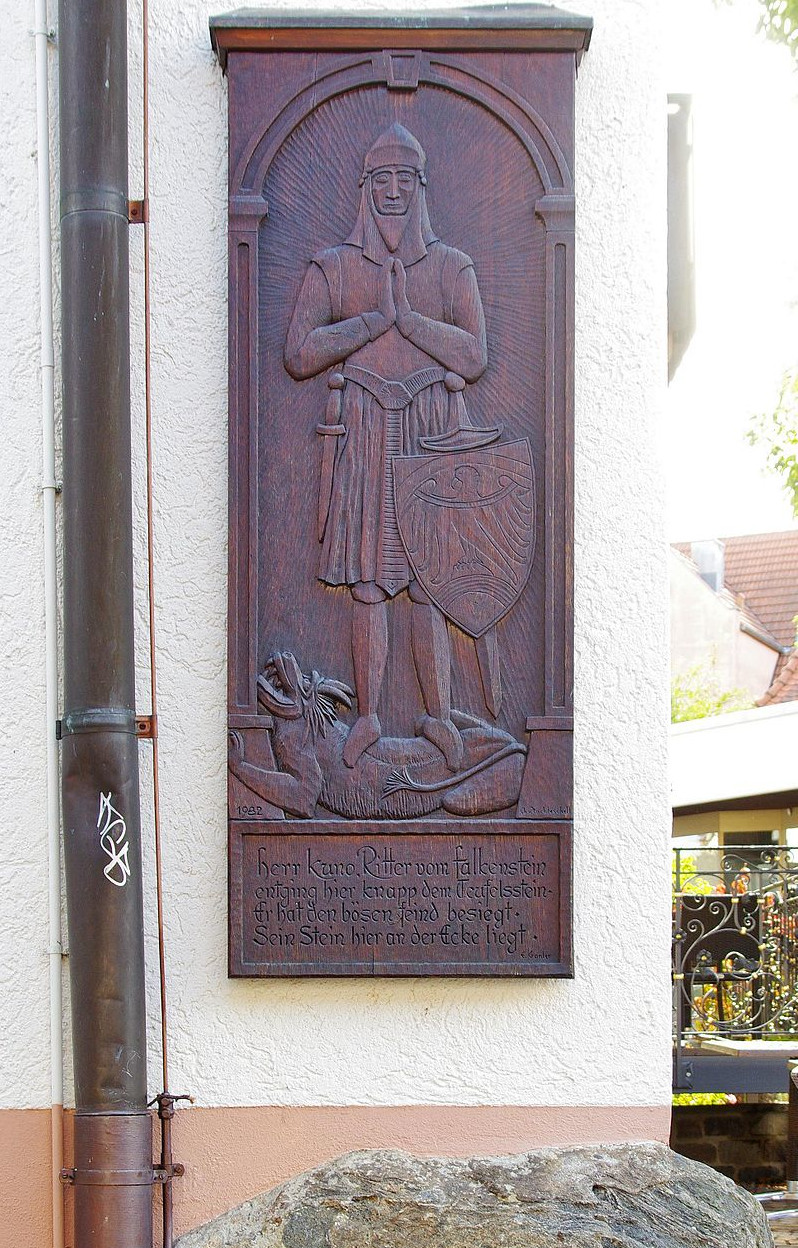
\includegraphics[width=\linewidth]{./figures/kuno_von_falkenstein_resized.jpg}
	\captionof{figure}{\iftoggle{isEnglish}{Kuno's gravestone in Kirchzarten}{}}
	\setlength{\parskip}{0.25cm}
\end{minipage}%
\hfill%
\vrule width 0.01cm
\hfill%
\begin{minipage}[t]{0.31\textwidth}
	\vspace{0cm}
	\setlength{\parskip}{0.25cm}

	\includegraphics[width=\linewidth]{./figures/höllental_historisch_resized.png}
	\captionof{figure}{\iftoggle{isEnglish}{Historical photo of the Ravenna Bridge}{}}
	\setlength{\parskip}{0.25cm}

	\iftoggle{isEnglish}{
	}{
	}

	\includegraphics[width=\linewidth]{./figures/ravenna_gorge_historical_resized.png}
	\captionof{figure}{\iftoggle{isEnglish}{Höllsteig and the Ravenna bridge around 1900}{}}
	\setlength{\parskip}{0.25cm}

	\iftoggle{isEnglish}{
  }{
  }

	\includegraphics[width=\linewidth]{./figures/höllentalbahn1900_resized.png}
	\captionof{figure}{\iftoggle{isEnglish}{The Höllentalbahn around 1900}{}}
	\setlength{\parskip}{0.25cm}
\end{minipage}%
\newpage
\begin{minipage}[t]{0.31\textwidth}
	\vspace{0cm}
	\setlength{\parskip}{0.25cm}

	\iftoggle{isEnglish}{
    Kuno von Falkenstein, known as the \enquote{crusader knight} of Höllental, died on 12 May 1343. Legend surrounds Kuno’s extraordinary return from the Crusades. Before departing in the early 14th century at the call of Bernard of Clairvaux, he asked his wife Ida to remain faithful for seven years, splitting his wedding ring and giving her one half. Captured, he eventually escaped but fell prey to a test by the Devil. The Devil promised to return him home disguised as a lion if he stayed awake, but hunger and exhaustion overcame him until a giant falcon appeared and kept him alert. At dawn on the seventh year the Devil set him down by the old inn Zum Rindsfuß, now Gasthaus Fortuna in Kirchzarten. Furious that Kuno had stayed awake, the Devil hurled a massive stone at him, but the stone smashed harmlessly into the corner of the inn. 

    Not long after, Idar on her way to marry Johann von Snewlin paused at the inn with her bridal procession. Kuno, veiled, approached for a drink of welcome wine. He dropped his ring half into the cup, Ida dropped hers, and the two pieces rejoined perfectly . At that moment she declared before Johann: \enquote{Here is my beloved husband whom I have been faithful to for seven years and whom God has returned to me in His mercy}. They returned to the church to renew their vows. Today Gasthaus Fortuna still displays a stone set into its corner, reputed to be the very Devil’s stone that struck the wall but failed to harm Kuno. A carved relief of Kuno is also mounted on the inn’s exterior, echoing the imagery of his grave slab and lion emblem.
	}{
	}
\end{minipage}%

\end{document}
